\section{Metodologia}
\label{sec:metodologia}

Após examinar diversos artigos e trabalhos científicos que abordaram redes veiculares, não foi identificado um padrão metodológico para a avaliação dessas redes. Normalmente, cada autor realiza a metodologia de acordo com as variáveis que se deseja avaliar. 

Os experimentos realizados neste trabalho baseiam-se em simulação. O uso de simulação justificou-se pela complexidade em se aplicar as técnicas propostas em uma grande quantidade de veículos, questões financeiras e relacionadas ao tempo para se testar o algoritmo em uma grande variedade de cenários também foram avaliadas.

Para comprovar a possibilidade da construção de um sistema baseado em agentes de software sobre uma VANET, foi elaborado um protótipo utilizando o trabalho \cite{santanaMestrado:2014} como referência e um cenário foi desenvolvido para avaliação.

A seção \ref{subsec:simulacao} descreve as etapas para a elaboração da simulação, onde será encontrado informações sobre o simulador, a estrutura do agente de software e o cenário utilizado para a simulação. As informações sobre o protótipo e o experimento em campo são descritas na seção \ref{subsec:prototipoExperimento}.

\subsection{Simulação}
\label{subsec:simulacao}

O desenvolvimento da simulação foi dividido em três etapas. A primeira etapa é a construção do cenário com o modelo de movimento, veículos e infraestrutura. A segunda etapa é o desenvolvimento dos agentes de software, e por último a fase de simulação. 

A simulação foi desenvolvida utilizando o simulador GRUBiX e executada em um notebook com configuração detalhada na tabela \ref{tab:configuracaoNotebook}.

\begin{table}[ht]
	\caption{Configuração do notebook utilizado nas simulações}
	\centering
	\begin{tabular}{|l|l|}
		\hline
		Sistema Operacional & Ubuntu Linux 10.10 \\ \hline
		Processador & Intel Core i7-2630QM 2.00GHz (6M Cache) \\ \hline
		Memória RAM & 8GB SSD \\ \hline
		Disco Rígido & 120 GB SSD \\ \hline 
	\end{tabular}

	\label{tab:configuracaoNotebook}
\end{table}

\subsubsection{Cenário}

O cenário é uma cidade dividida em quadras seguindo o modelo de movimento \emph{Manhattan}. Nessa cidade possuem veículos que percorrem as quadras. Alguns cruzamentos possuem uma infraestrutura e elas estão conectadas através de cabos. 

A figura \ref{fig:modeloMovimentoManhattan} apresenta um esboço do cenário onde pode-se observar as ruas, os veículos e a infraestrutura. Esse cenário é utilizado em todas simulações, entretanto a infraestrutura é desativada quando não é utilizada.

\begin{figure}[htbp]
	\centering
	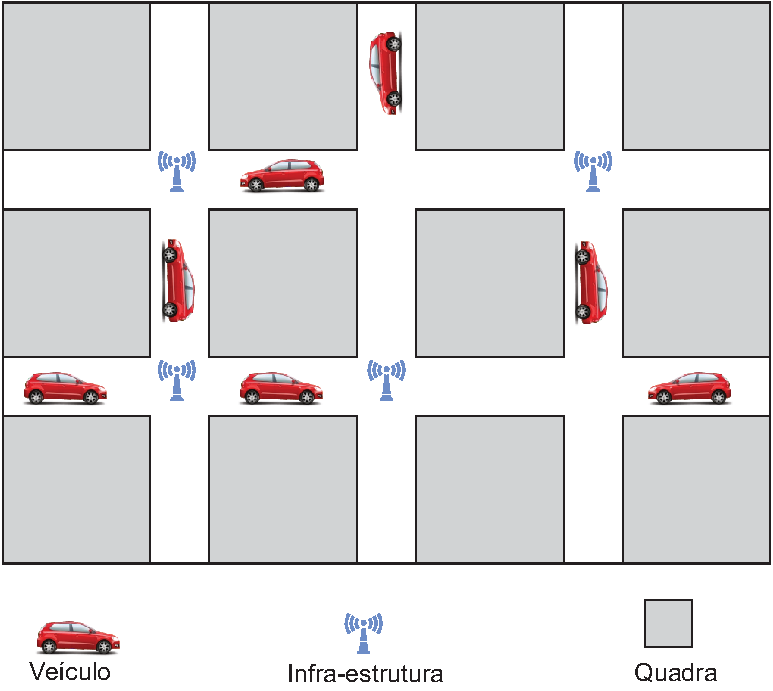
\includegraphics[scale=0.7]{metodologia/figuras/modeloMovimentoManhattan.pdf}
	\caption{Modelo de cidade utilizado.}
	\label{fig:modeloMovimentoManhattan}
\end{figure}

O comprimento e a largura da região de simulação são levados em consideração na construção do cenário. As linhas horizontais e verticais são as ruas e o cruzamento delas são as quadras. Para obter a quantidade de ruas horizontais e verticais são utilizadas as Equações \ref{eq:equacaoQuantidadeRuasHorizontal} e \ref{eq:equacaoQuantidadeRuasVertical}.

\begin{equation}
	\label{eq:equacaoQuantidadeRuasHorizontal}
	Q_{rh} = {A_{at} \over A_{aq}}
\end{equation} 

\begin{tabular}{ l c r} 
	Onde:\\
	Q\tiny rh \normalsize= quantidade de ruas na horizontal \\
	A\tiny at \normalsize= altura total do cenário \\
	A\tiny aq \normalsize= altura das quadras\\
\end{tabular}

\begin{equation} 
	\label{eq:equacaoQuantidadeRuasVertical}
	Q_{rv} = {L_{lt} \over L_{lq}} 
\end{equation}

\begin{tabular}{ l c r}
	Onde:\\ 
	Q\tiny rh \normalsize= quantidade de ruas na vertical \\
	L\tiny lt \normalsize= largura total do cenário \\
	L\tiny lq \normalsize= largura das quadras\\
\end{tabular}

\paragraph{Veículos e infraestrutura}

O agente necessita que os nós (veículos e a infraestrutura) tenham dois recursos fundamentais para o seu funcionamento: a capacidade de comunicação; e o agente deve conseguir executar suas instruções. Na simulação todos os nós possuem essa competência.

Quando um agente chega em um nó, ele logo executa a suas instruções. No simulador o nó executa um evento para verificar se existe algum agente hospedado nele. Se existir o evento retorna um objeto que deve implementar a interface agente que se encontra no Anexo \ref{app:agente}. Com o objeto o nó executa o método \texttt{execute()}. As classes do programa em Java  que simulam o comportamento do nó se encontra no Anexo \ref{app:comportamentoNo}. O Anexo \ref{app:movimento} descreve a classe java que implementa o modelo de movimento.

Todos os veículos e infraestruturas possuem o mesmo comportamento em relação ao agente. Por outro lado, eles possuem comportamentos diferentes em relação ao ambiente. Primeiramente os veículos possuem a capacidade de locomoção. Embora a infraestrutura não possua essa capacidade, todas elas estão conectadas. Em outras palavras, quando um agente está em uma infraestrutura ele não consegue se locomover porém consegue se comunicar com todas as outras infraestruturas espalhadas pelo cenário. 

Ao iniciar a simulação os veículos e as infraestruturas são distribuídos entre os cruzamentos de maneira aleatória. 

O Algoritmo \ref{lst:algoritmoComportamentoNos} de locomoção leva em consideração a equação da reta que representa a rua. Isto significa que quando o veículo está em uma rua do tipo horizontal ele se movimenta em \emph{X} e quando estiver em uma rua do tipo vertical o veículo se movimenta em \emph{Y}. Para simular a velocidade quando um veículo entra em uma rua, o tipo dela é verificado e então soma ou subtrai um valor da posição atual dele.

\begin{algorithm}
	\scriptsize
	\Inicio{
		$nos \gets pegarListaNos()$\;
		$i \gets 0$\;
		\Repita{i == nos.length}{
			\uIf{nos[i].eVeiculo()}{
				pontoProximoCruzamento = nos[i].pegarCruzamentoMaisProximo()\;
				distancia = pontoProximoCruzamento.calcularDistancia(nos[i].posicao)\;
				\uIf{distancia < nos[i].velocidade}{
					nos[i].velocidade = distancia\;
				}
				\Else{
					\uIf{distancia == 0}{
						nos[i].mudarDirecao()\;
					}
					\Else{
						nos[i].andar()\; 
					}
				}
			}
			\uIf{nos[i].possuiAgente()}{
				nos[i].pegarAgente().execute()\;
			}
			i++\;
		} 
	}
	\caption{Algoritmo movimento dos nós.}
	\label{lst:algoritmoComportamentoNos}
\end{algorithm} 

Quando a velocidade do veículo é maior que a distância entre a posição atual dele e de um cruzamento, a sua velocidade diminui até chegar em zero. Isto significa que o veículo chegou em um cruzamento, então o veículo deve decidir entre continuar, virar para esquerda, virar para direita ou voltar. Cada direção possui uma probabilidade como demonstra a Tabela \ref{tab:probabilidadeEscolhaDirecao}.

No caso da infraestrutura a velocidade é sempre zero. Assim elas utilizam o mesmo algoritmo dos veículos porém não mudam de posição.

\begin{table}[ht]
	\caption{Probabilidade do veículo escolher uma direção}
	\centering
	\begin{tabular}{ | l | c | r}
		\hline
		Frente & 50\% \\ \hline
		Direita & 20\% \\ \hline
		Esquerda & 20\% \\ \hline
		Voltar & 10\% \\ \hline 
	\end{tabular}
	\label{tab:probabilidadeEscolhaDirecao}
\end{table}

O Algoritmo \ref{lst:algoritmoAproximacaoRuas} demonstra que em cada movimento do veículo são calculadas as distâncias entre a sua posição atual e de todos os cruzamentos contrários ao tipo de rua que o veículo está locomovendo.
Por exemplo, quando um veículo se locomove em uma rua horizontal, a cada movimento o algoritmo calcula as distâncias entre a posição do veículo e as ruas verticais.

\begin{algorithm}
	\scriptsize
	\Inicio{
		\Entrada{O nó a ser testado}
		$i \gets 0$\;
		\uIf{no.tipoRua == horizontal}{
			$y \gets no.posicao.getY()$\;
			\Repita{$i < Q_{rh}$}{
				$y_{rua} \gets A_{aq}(1 + i)$ \;
				\uIf{$y_{rua} - y < no.velocidade$}{
					retorna $y_{rua} - y$ \;
				}
				i++\;
			}
		}
		\Else{
			\uIf{no.tipoRua == vertical}{
				$x \gets no.posicao.getX()$\;
				\Repita{$i < Q_{rv}$}{
					$x_{rua} \gets L_{lq}(1 + i)$ \;
					\uIf{$x_{rua} - x < no.velocidade$}{
						retorna $x_{ruax} - x$ \;
					}
					i++\;
				}
			}
		} 
	}
	\caption{Algoritmo que identifica a aproximação com um cruzamento.}
	\label{lst:algoritmoAproximacaoRuas}
\end{algorithm}

Para definir as ruas horizontais é utilizado a Equação \ref{eq:equacaoParaEncontraRuasHorizontais} que é a equação da reta quando a reta cruza o eixo \emph{Y}.

A Equação \ref{eq:equacaoParaEncontraRuasVerticais} é utilizada para definir as ruas verticais. Todas as ruas horizontais se cruzam com as ruas verticais, então para descobrir um cruzamento é necessário indicar o número da rua nas Equações \ref{eq:equacaoParaEncontraRuasHorizontais} e \ref{eq:equacaoParaEncontraRuasVerticais} respectivamente. Com isso é optido um ponto que corresponde ao cruzamento.

\begin{equation} 
	\label{eq:equacaoParaEncontraRuasHorizontais}
	Y = A_{aq}(1+N_{horizontral}) 
\end{equation}

\begin{tabular}{ l c r}
	Onde:\\ 
	Y = posição da rua \\
	A\tiny aq \normalsize= altura das quadras\\
	N\tiny horizontal \normalsize=número de quadras onde $N_{horizontal} \in I, 0 \leq N_{horizontal} < Q_{rv}$\\
\end{tabular}

\begin{equation} 
	\label{eq:equacaoParaEncontraRuasVerticais}
	X = L_{lq}(1+N_{vertical}) 
\end{equation}

\begin{tabular}{ l l}
	Onde:\\ 
	X = posição da rua \\
	L\tiny lq \normalsize= largura das quadras\\
	N\tiny vertical \normalsize=número de quadras onde $N_{vertical} \in I, 0 \leq N_{vertical} < Q_{rv}$\\
\end{tabular}

\subsubsection{Agente de Software}

Foi utilizado \cite{Freitas:2011} como referência para a construção do agente de software. A missão do agente é permanecer dentro de uma região (região alvo) no cenário. A região é definida por dois pontos, sendo um limite superior e outro o limite inferior, como demonstra a Figura \ref{fig:regiaoAlvo}. 

\begin{figure}[htbp]
	\centering
	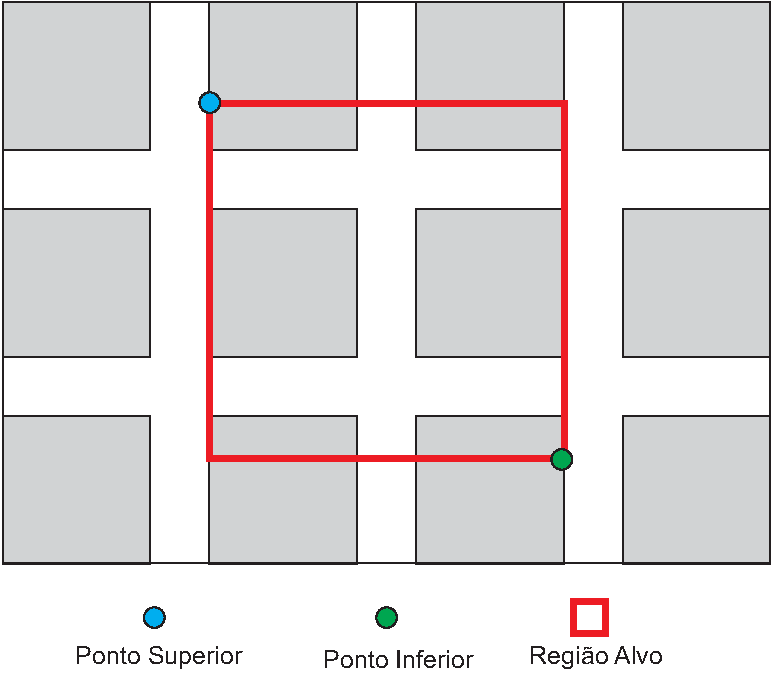
\includegraphics[scale=0.7]{metodologia/figuras/regiaoAlvo.pdf}
	\caption{Região Alvo.}
	\label{fig:regiaoAlvo}
\end{figure}

Para a simulação foram criados dois tipos de agentes. O agente que deve se manter dentro da região alvo é o agente principal. O agente principal pode criar um tipo de agente mais simples, o \emph{mini-agente}, que é responsável por buscar nós que possam propiciar ao agente principal maior possibilidade de finalizar a sua missão.

Quando a simulação inicia é escolhido um nó aleatoriamente para receber um agente principal. Então o nó executa as instruções do agente. Para o funcionamento dessa arquitetura o agente precisa possuir uma interface onde o veículo consiga acessar as instruções do agente. Os nós também devem ter uma interface onde o agente consiga acessar recursos necessários para o seu funcionamento. Nesse trabalho, os nós possuem três recursos disponíveis:

\begin{itemize}
	\item Posição atual
	\item Posição com o destino do nó
	\item Comunicação com os nós vizinhos
\end{itemize} 

Na Figura \ref{fig:umlAtores} pode-se visualizar a arquitetura das simulações. Essa arquitetura permite adicionar mais atores na simulação, por exemplo, agentes como missões diferentes ou até mesmo uma pessoa com algum equipamento que permita o transporte dos agentes. Assim, possibilita-se ao agente acessar regiões antes impossíveis para acesso de veículos. 

\begin{figure}[htbp]
	\centering
	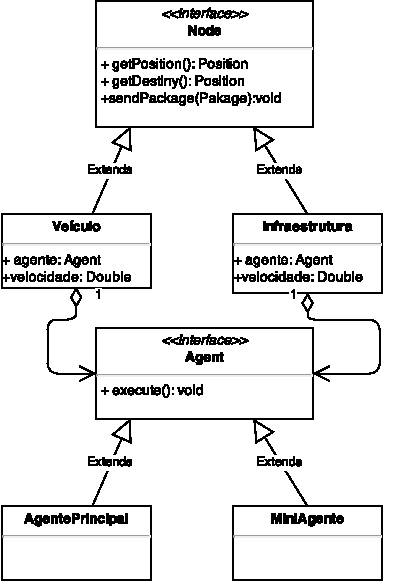
\includegraphics[scale=0.8]{metodologia/figuras/umlAtores.pdf}
	\caption{Diagrama UML com a relação entre as entidades.}
	\label{fig:umlAtores}
\end{figure}

A missão do agente é alcançar a região alvo e permanecer nela. Para isto, o agente deve conhecê-la. Então a primeira ação do agente é solicitar ao nó onde ele está hospedado a sua posição. Se o veículo estiver na região alvo o algoritmo termina a sua execução, e nesse momento poderia realizar outras atividades como recolher dados ou disseminar propaganda.

Caso a posição do nó não está no interior da região alvo, o agente precisa procurar um hóspede mais apropriado. Para isso é criado um segundo agente, mais simples que o primeiro, com a missão de procurar entre os nós vizinhos um mais apropriado. O Algoritmo \ref{lst:algoritmoAgentePrincipal} descreve o funcionamento do agente principal.

\begin{algorithm}
	\scriptsize
	\Inicio{
		\Repita{$no.agentePrincipal \neq vazio$}{
			$regiaoAlvo \gets pegarRegiaoAlvo()$\;
			$posicaoNo \gets no.pegarPosicao()$\;
			$destinoNo \gets no.pegarDestino()$\;
			\uIf{$posicaoNo \in regiaoAlvo$}{
				executarTarefasDaRegiaoAlvo()\;
			}
			\Else{
				$miniAgente \gets criarMiniAgente(posicaoNo, destinoNo, regiaoAlvo)$\;
				$mensagem \gets no.enviarMensagem()$\;
				$reposta = escutarReposta(mensagem)$\;

				\uIf{reposta = vazio}{
					executarTarefasForaRegiaoAlvo()\;
				}
				\Else{
					no.enviarMensagem(agentePrincipal, reposta.idImovelSelecionado())\;
				}
			}
			hibernarPeriodo()\; 
		} 
	}
	\caption{Algoritmo do Agente Principal.}
	\label{lst:algoritmoAgentePrincipal}
	\end{algorithm}

Cada nó vizinho recebe uma cópia do \emph{mini-agente} e o executa. Na estrutura do \emph{mini-agente} contém a região alvo e a distância do destino com a região alvo. Esses dados são comparados pelo \emph{mini-agente} com os dados dos nós que o receberam. Caso algum nó tenha uma condição melhor que o nó onde o agente principal está hospedado o \emph{mini-agente} envia um sinal avisando o agente principal para ele migrar. Após finalizar a missão o \emph{mini-agente} é descartado. O funcionamento do \emph{mini-agente} é reproduzido pelo algoritmo \ref{lst:algoritmoMiniAgente}.

\begin{algorithm}
	\scriptsize
	\Inicio{
		\Entrada{posicaoNoHospedeiro, destinoNoHospedeiro, regiaoAlvo}
		$distanciaRegiaoAlvoDestinoNoHospedeiro \gets regiaoAlvo.calcularDistancia(destinoHospedeiro)$\;
		$distanciaRegiaoAlvoDestinoNo \gets regiaoAlvo.calcularDistancia(no.destino)$\;
		\uIf{$no.posicao \in regiaoAlvo$}{
			no.enviarSinal(no.id)\;
		}
		\Else{

			\uIf{$no.destino \in regiaoAlvo$}{
				no.enviarSinal(no.id)\;
			}
			\Else{
				\uIf{$distanciaRegiaoAlvoDestinoNoHospedeiro < distanciaRegiaoAlvoDestinoNo$}{
					no.enviarSinal(no.id)\;
				}
			}
		}
		no.removerMiniAgente()\;s
	}
	\caption{Algoritmo do Mini-agente.}
	\label{lst:algoritmoMiniAgente}
\end{algorithm}

Durante a seleção três perguntas devem ser respondidas e, se uma das respostas for afirmativa, o \emph{mini-agente} envia o sinal para o agente principal migrar:

\begin{enumerate}
	\item Nó está dentro da região alvo? (Figura \ref{fig:veiculoSelecionadoDentroRA})
	\item Destino do nó é dentro da região alvo? (Figura \ref{fig:destinoVeiculoSelecionadoDentroRA})
	\item Destino do nó é mais próximo da região alvo? (Figura \ref{fig:destinoVeiculoSelecionadoProximoRA})
\end{enumerate}

\begin{figure}[htbp]
	\centering
	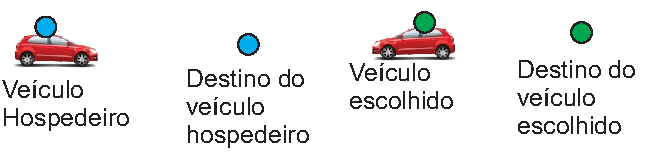
\includegraphics[scale=0.7]{metodologia/figuras/legendaSelecaoMelhorVeiculo.pdf}
\end{figure}

\begin{figure}[htbp]
	\centering
	\begin{minipage}{0.50\textwidth}
		\centering
		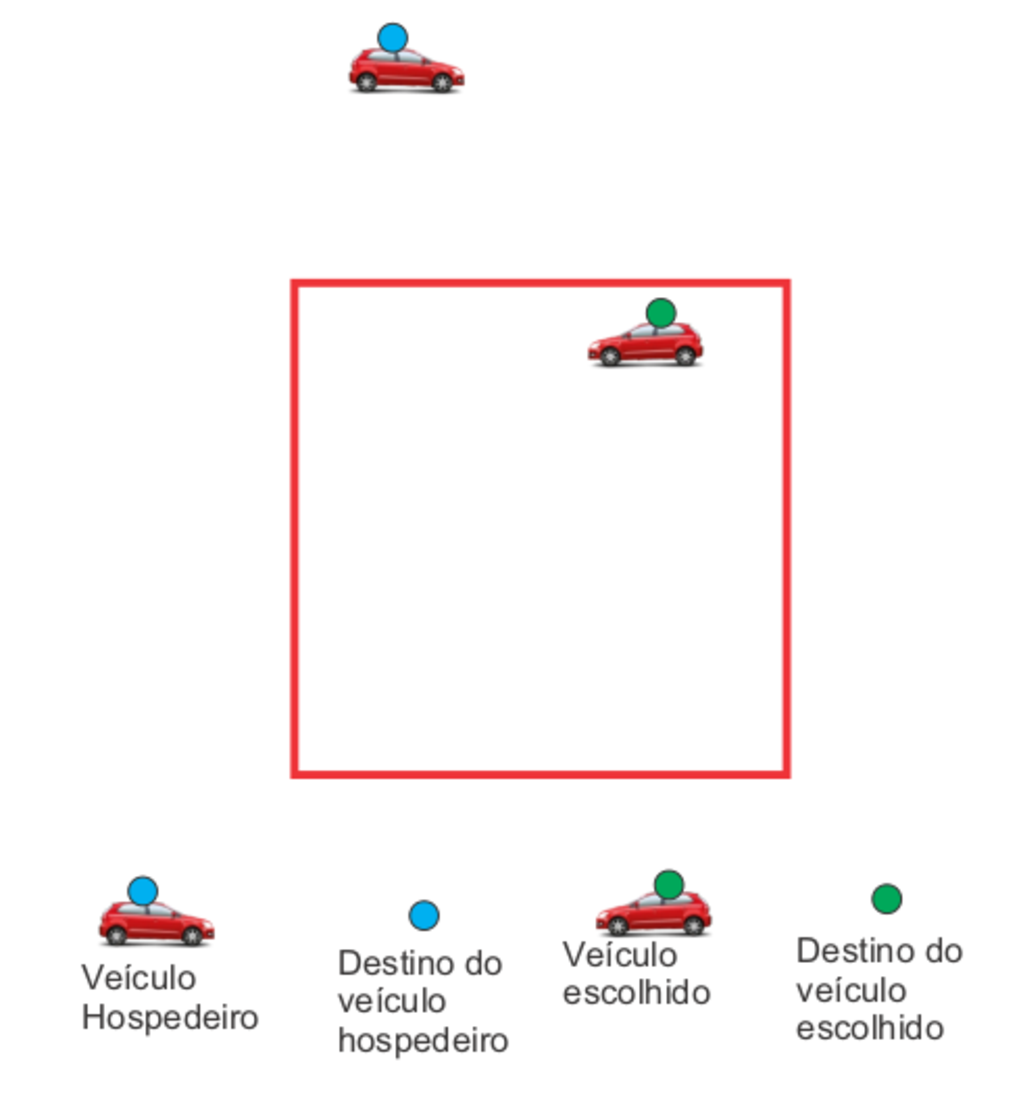
\includegraphics[scale=0.5]{metodologia/figuras/veiculoSelecionadoDentroRA.pdf}
		\captionof{figure}{Veículo dentro da Região Alvo.}
		\label{fig:veiculoSelecionadoDentroRA}
	\end{minipage}%
	\begin{minipage}{0.50\textwidth}
		\centering
		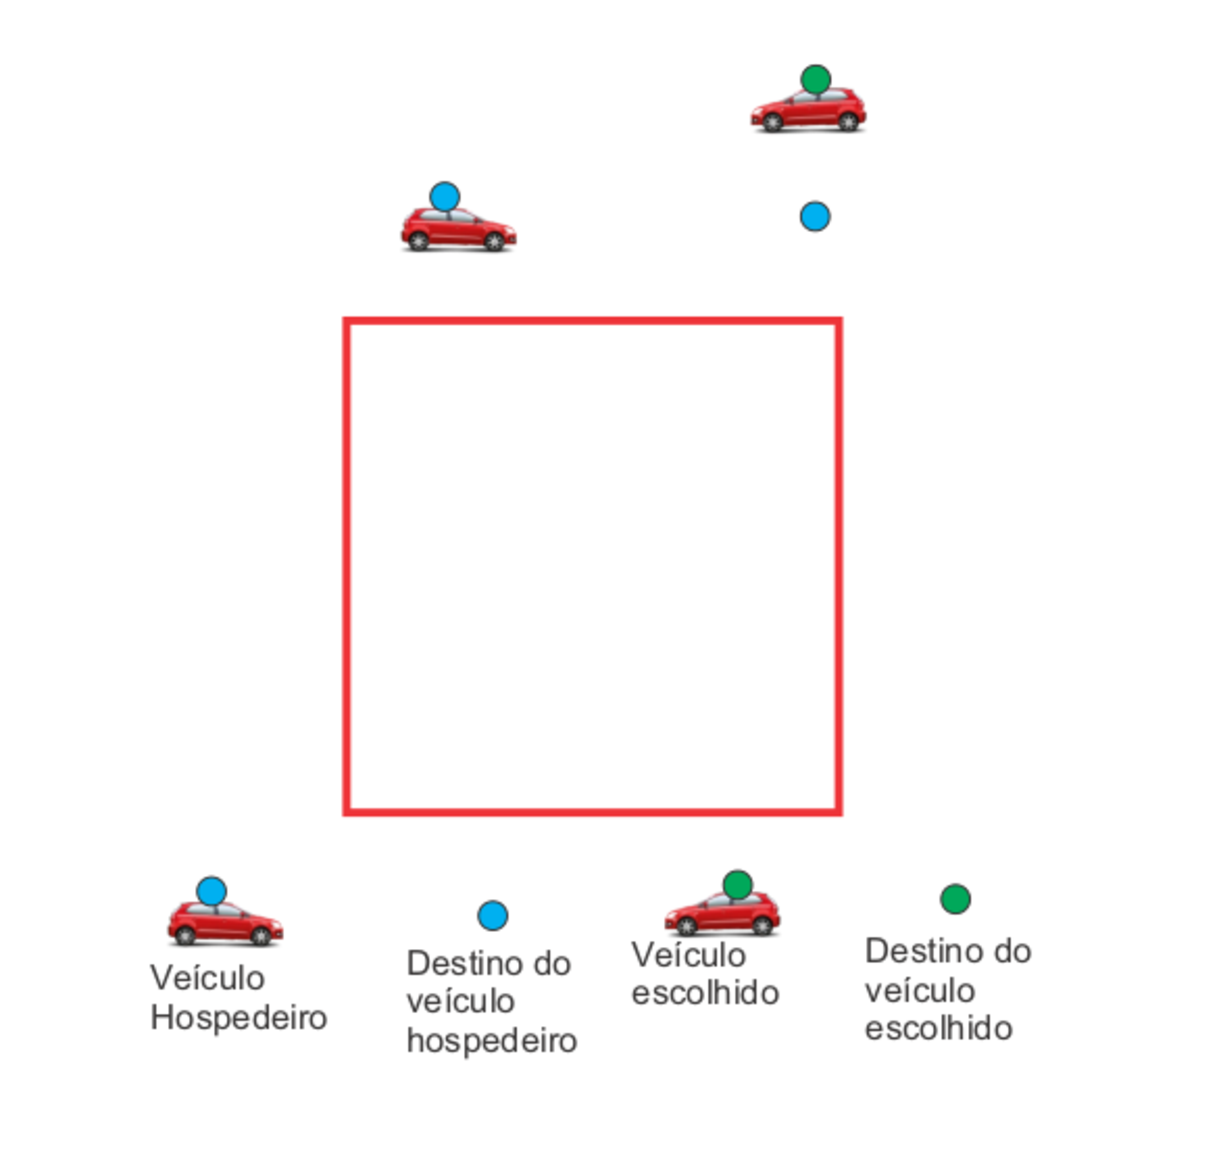
\includegraphics[scale=0.5]{metodologia/figuras/destinoVeiculoSelecionadoDentroRA.pdf}
		\captionof{figure}{Destino veículo dentro da Região Alvo.}
		\label{fig:destinoVeiculoSelecionadoDentroRA}
	\end{minipage}
	\begin{minipage}{0.50\textwidth}
		\centering
		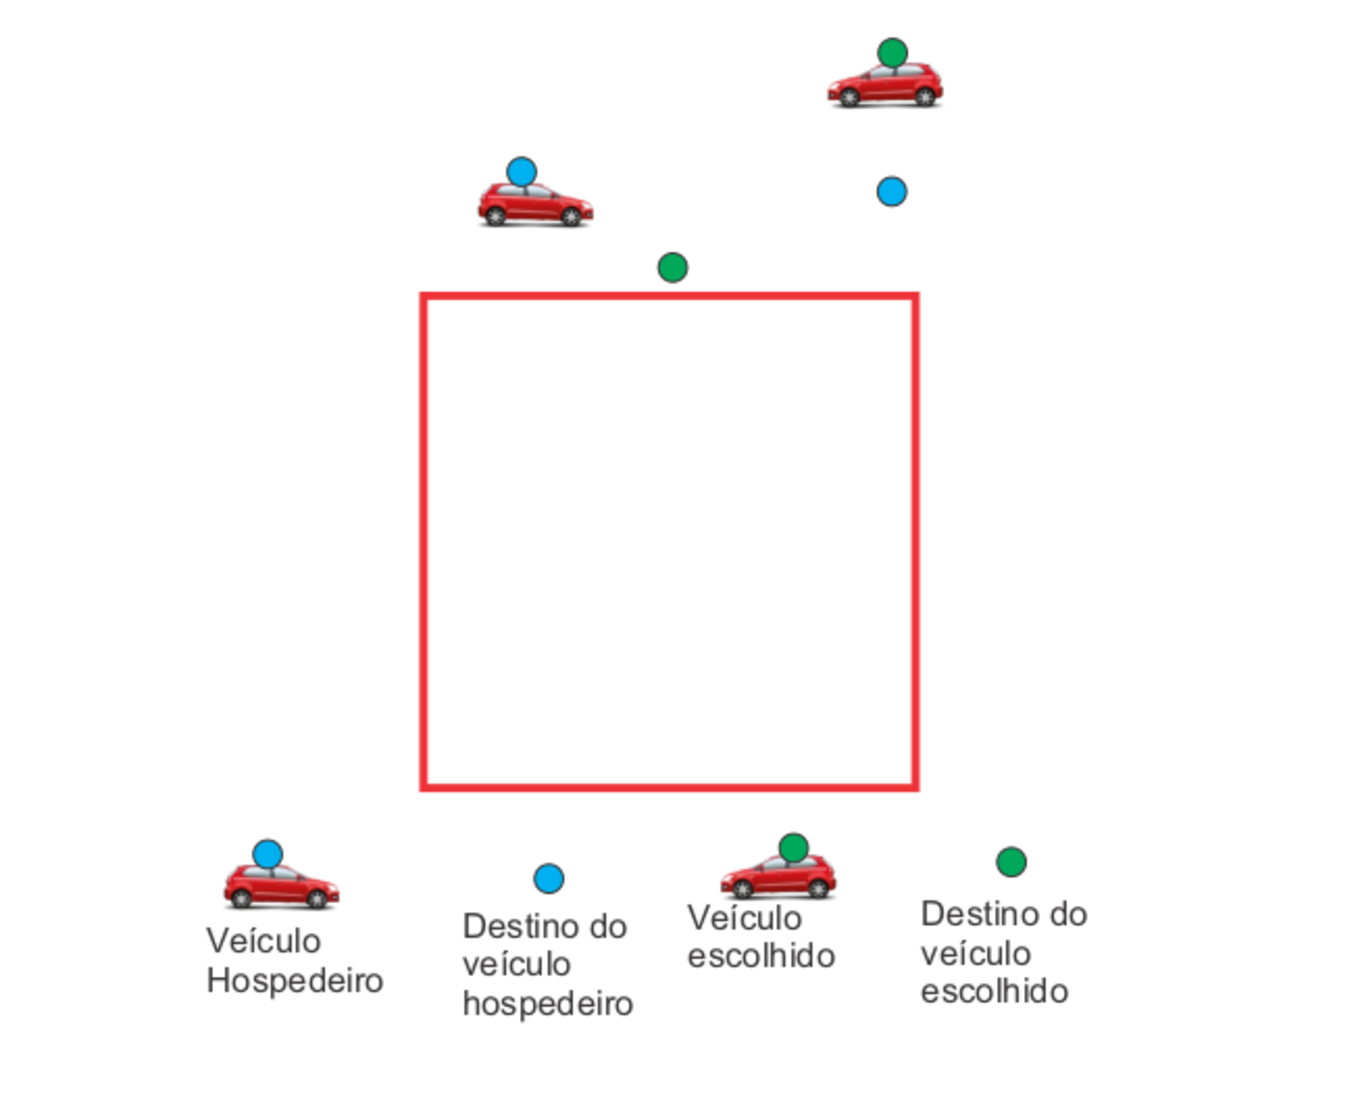
\includegraphics[scale=0.5]{metodologia/figuras/destinoVeiculoSelecionadoProximoRA.pdf}
		\captionof{figure}{Destino do veículo selecionado dentro da Região Alvo.}
		\label{fig:destinoVeiculoSelecionadoProximoRA}
	\end{minipage}
\end{figure}

O primeiro sinal que alcançar o agente principal, ele realiza a migração para o nó que enviou o sinal. Essa abordagem é utilizada por dois motivos:

\begin{description}
	\item[Primeiro:] O sinal contendo somente o identificador do nó possui poucos bytes.
	\item[Segundo:] Elimina a necessidade do desenvolvimento um mecanismo para esperar que todos os \emph{mini-agente} executem a sua missão e só depois tomar a decisão de escolher o melhor nó.
\end{description}

Na simulação que a infraestrutura está ativada, ela pode replicar o \emph{mini-agente} para todos os outros nós próximos 
às infraestruturas espalhadas pelo cenário, aumentando a abrangência da busca. Se um nó distante for escolhido, o agente principal pode utilizar a infraestrutura para alcançá-lo. A Figura \ref{fig:exemploComInfraestrutura} demonstra uma situação onde o \emph{mini-agente} encontra uma infraestrutura.

\begin{figure}[htbp]
	\centering
	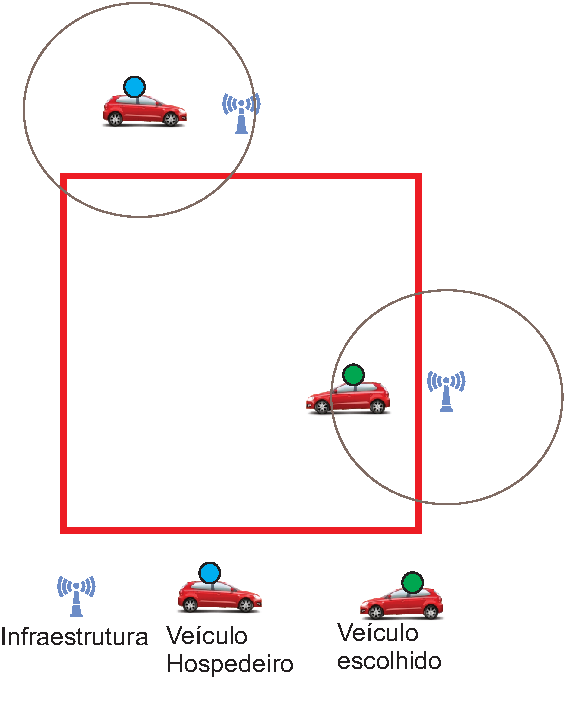
\includegraphics[scale=0.5]{metodologia/figuras/exemploComInfraestrutura.pdf}
	\label{fig:exemploComInfraestrutura}
	\caption{Exemplo com infraestrutura.}
\end{figure}

Para não congestionar a rede, o agente principal deve evitar procurar novos nós por um período de tempo, e durante esse período ele pode executar outras tarefas. Esse comportamento pode ser repetido infinitamente ou o agente pode ter um tempo determinado para executar a sua missão. Ao fim desse tempo, o agente deixa de existir.

\subsubsection{Realizar simulação}

O objetivo da simulação é averiguar se a adição de uma infraestrutura melhora a locomoção dos agentes de software, favorecendo que ele desempenhe a sua missão. Após o desenvolvimento e testes do cenário e de todos os atores da simulação é necessário configurar o simulador. As varáveis que o simulador GRUbiX utiliza são: quantidade dos nós, alcance do sinal, largura e altura do cenário. 

As variáveis largura e altura do cenário são constantes em 120 metros. Por outro lado, a quantidade de nós e alcance de cada nó são variáveis. Essa variação permite simular o comportamento do agente em ambientes com alta e baixa densidade de veículos. Com a altura e largura do cenário é possível obter as quadras. Elas possuem 10 metros de altura e 10 de largura, totalizando 144 quadras.

Após configurar as variáveis de ambiente do GRUBiX é necessário configurar os atores da simulação. Os atores da simulação são: veículos, infraestruturas, agente principal e o agente secundário. As variáveis dos nós que representam os veículos são o alcance e a velocidade. Os nós que representam as infraestruturas possuem o mesmo alcance dos veículos, porém a velocidade é nula e também podem ser ativados e desativados. O agente principal só precisa conhecer a região alvo, onde o ponto superior é S(80,100) e o inferior é I(100,80) sendo a escala em metros.  

Então foram modeladas vinte e quatro situações para serem simuladas. Elas consistem em doze com a infraestrutura ligada e outras doze com a infraestrutura desligada. A Tabela \ref{tab:resumoConfiguracaoSimulacao} apresenta um resumo das configurações simuladas. 

\begin{table}[ht]
	\caption{Resumo das configurações da simulação}
	\centering
	\begin{tabular}{| l | l | l | l | l | l | l | l | l |}
		\hline
		Infraestrutura & \multicolumn{4}{|c|}{Ativada} & \multicolumn{4}{|c|}{Desativada} \\ \hline
		Quantidade de nós & 25 & 50 & 75 & 100 & 25 & 50 & 75 & 100 \\ \hline
		Alcance dos nós (metros) & 5 & 5 & 5 & 5 & 5 & 5 & 5 & 5 \\
		Alcance dos nós (metros)& 10 & 10 & 10 & 10 & 10 & 10 & 10 & 10 \\
		Alcance dos nós (metros)& 15 & 15 & 15 & 15 & 15 & 15 & 15 & 15 \\
		\hline 
	\end{tabular}
	\label{tab:resumoConfiguracaoSimulacao}
\end{table}

O simulador permite uma visualização da simulação como apresenta a Figura \ref{fig:visulizacaoSimulador}. Nela as linhas representam as ruas, os pontos amarelos são os veículos e os vermelhos são a infraestrutura. Nas simulações, quando a infraestrutura está ativada, cinco nós que seriam veículos se tornam infraestrutura e a sua velocidade mantém nula. Quando a infraestrutura está desligada os nós continuam sendo veículos. Exemplificando: com a infraestrutura ligada, quando existir vinte e cinco nós, cinco nós são infraestrutura e o restante veículos. Por outro lado, quando a infraestrutura estiver desligada, todos os nós são veículos.

\begin{figure}[htbp]
	\centering
	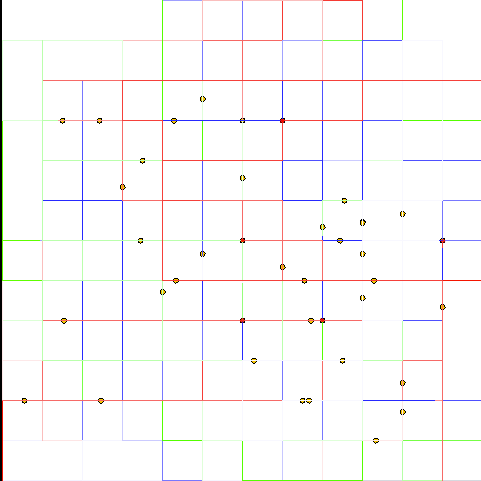
\includegraphics[scale=0.4]{metodologia/figuras/simulacaoGrubix.png}
	\caption{Visualização no simulador.}
	\label{fig:visulizacaoSimulador}
\end{figure}

Foram realizadas mil simulações para cada uma das vinte e quatro situações totalizando vinte e quatro mil simulações. Os dados recolhidos foram o tempo de simulação e o tempo que o agente permaneceu dentro da região alvo.  

Com esses dados é possível obter a porcentagem de tempo que o agente principal permaneceu na região alvo e o impacto que cada variável tem no desempenho do agente em cumprir a missão. Com os resultados finais foram calculados desvio padrão, variância e assim analisados.


\section{Metodologia do Protótipo}
\label{sec:prototipoExperimento}

Um protótipo foi desenvolvido para avaliar o uso dos agentes fora do ambiente virtual. O objetivo desta fase é recolher dados sobre a latência e taxa de perda do agente. A latência é importante para alguns tipos aplicações como por exemplo para detectar colisão \cite{santanaMestrado:2014}. Assim, essas informações são importantes para identificar quais os tipos de aplicações os agentes são melhores empregados. Uma rede para ser bem sucedida com a utilização dos agentes de software necessita mante-los ativo até o fim de sua missão.A Figura \ref{fig:noInstaladoVeiculo} pode-se visualizar um nó instalado em um veículo.

\begin{figure}[htbp]
	\centering
	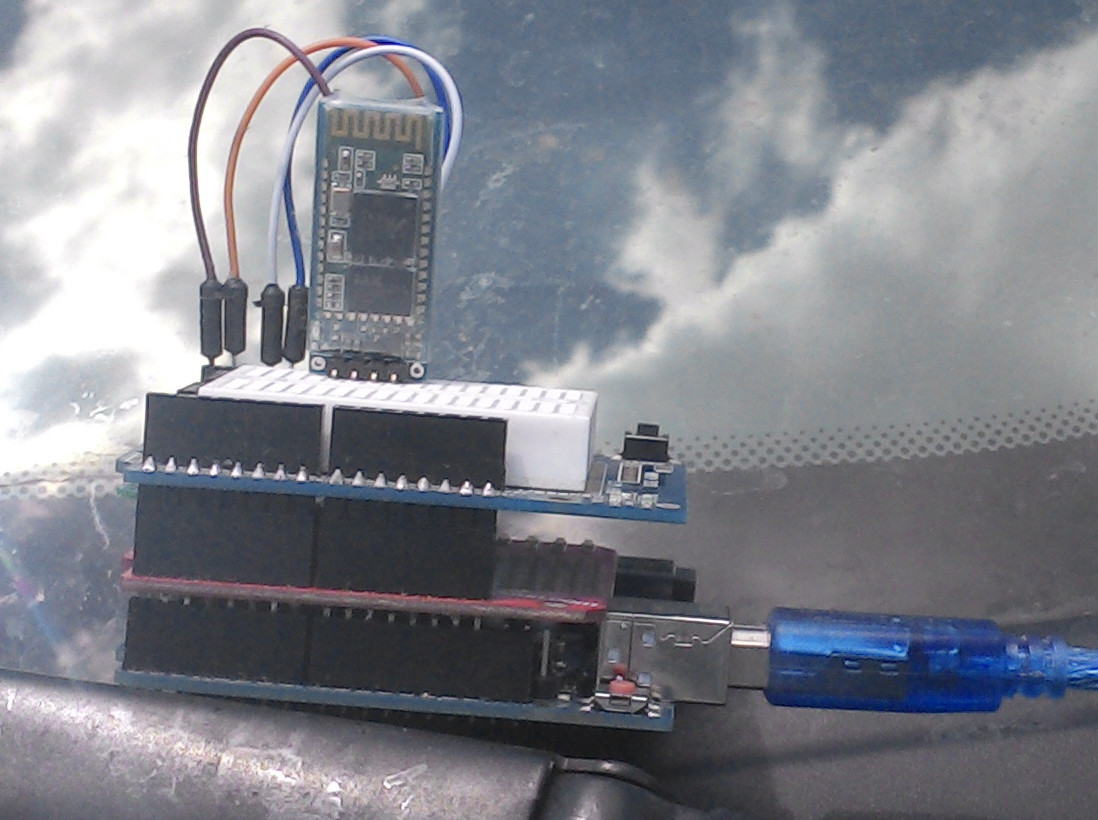
\includegraphics[scale=0.2]{metodologia/figuras/noInstaladoVeiculo.jpg}
	\caption{Nó instalado em um veículo.}
	\label{fig:noInstaladoVeiculo}
\end{figure}

O experimento utiliza três nós, onde dois nós são para os veículos e um desempenha o papel de infraestrutura. A estrutura dos nós foi reaproveitada do trabalho \cite{santanaMestrado:2014}. Os equipamentos necessários para a construção dos nós podem ser visualizados na Tabela \ref{tab:componentesPrototipo}. 

\begin{table}[ht]
	\caption{Equipamentos utilizados no experimento.}
	\centering
	\begin{tabular}{|l|l|}
		\hline
		Equipamento & Quantidade \\ \hline
		Notebook & 1 \\ \hline 
		Módulo bluetooth modelos JY-MCU & 2 \\ \hline
		Arduíno UNO & 2 \\ \hline
		Xbee shield & 2 \\ \hline
		Mini protoboard 170 pontos & 2 \\ \hline
		Xbee S1 & 3 \\ \hline
		XBee Explorer USB Adapter & 1 \\ \hline 
		Motorola RAZR I & 1 \\ \hline
		Motorola Moto G & 1 \\ \hline
	\end{tabular}
	\label{tab:componentesPrototipo}
\end{table}

Ao iniciar o experimento é introduzido um agente em um dos nós. Então o agente deve migrar sempre que encontrar um outro nó.

\subsection{Arquitetura do nó}

A Figura \ref{fig:arquiteturaPrototipoInfraestrtura} demonstra a arquitetura da infraestrutura que utiliza um Xbee e um XBee Explorer USB Adapter conectado em um notebook.

\begin{figure}[htbp]
	\centering
	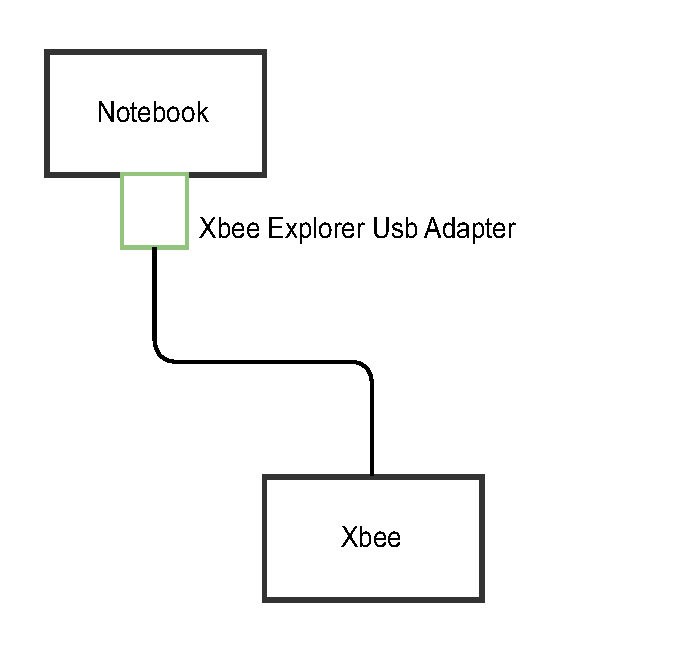
\includegraphics[scale=0.5]{metodologia/figuras/arquiteturaPrototipoInfraestrtura.pdf}
	\caption{Arquitetura da infraestrutura.}
	\label{fig:arquiteturaPrototipoInfraestrtura}
\end{figure}

O agente fica hospedado no smartphone, o arduino serve somente como interface entre o smartphone e o módulo Xbee. A comunicação entre o arduino e o smartphone acontece através do bluetooth. 

O smartphone acolhe o agente por que possui um ambiente mais rico em recursos do que o arduino, isto significa que o smartphone possui GPS, mais memória e outros recursos para que o agente possa desempenhar a sua missão, a Figura \ref{fig:arquiteturaPrototipoVeiculo} ilustra a estrutura do nó que atua nos veículos. 

\begin{figure}[htbp]
	\centering
	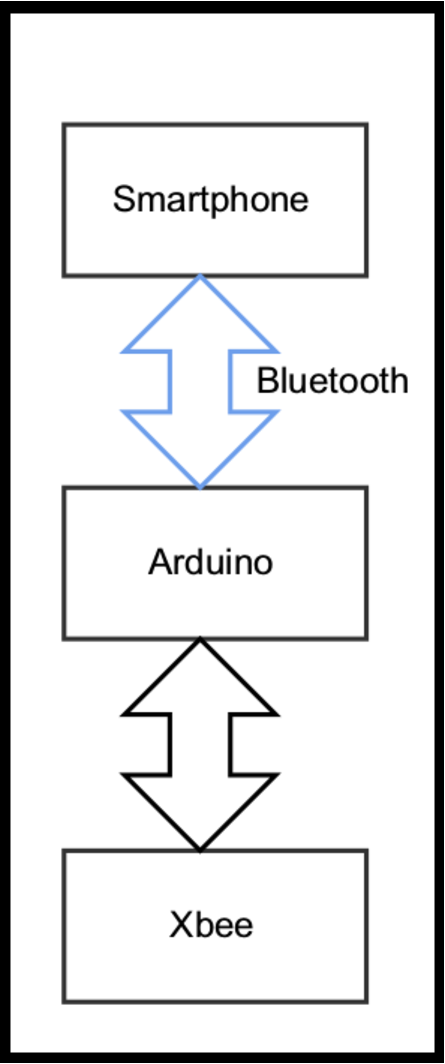
\includegraphics[scale=0.5]{metodologia/figuras/arquiteturaPrototipoVeiculo.pdf}
	\caption{Estrutura do nó no veículo.}
	\label{fig:arquiteturaPrototipoVeiculo}
\end{figure}

Para sincronizar o relógio dos smartphones utilizados no experimento foi utilizado o aplicativo NTPSync (\cite{Ntpsync:2015}), que é um aplicativo simples para sincronizar o tempo. Manter o relógio sincronizado é importante para medir a latência com precisão. 


Para hospedar o agente foi desenvolvido um aplicativo Android, esse aplicativo fornece ao agente os mecanismos necessários para realizar a sua missão. Através dele o agente consegue acessar o GPS, o bluetooth e a tela do smartphone. No display do aplicativo tem um alerta que informa se existe algum agente hospedado no smartphone e um botão para criar novos agentes. A Figura \ref{fig:appScreen} demonstra a tela do aplicativo responsável pelo agente.

\begin{figure}[htbp]
	\centering
	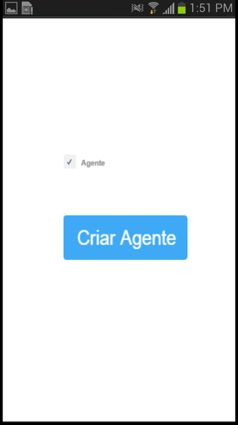
\includegraphics[scale=0.5]{metodologia/figuras/appScreen.jpg}
	\caption{Tela do aplicativo.}
	\label{fig:appScreen}
\end{figure}

Esse aplicativo também realiza a coleta dos dados em arquivo. Os dados coletados são a hora que o agente migrou, a hora que recebeu um agente em milisegundo. Então para calcular a latência é a subtração da hora de quando o novo hospede recebeu o agente e a hora que o agente iniciou a migração no antigo hospede.

\subsection{Agente}

A missão do agente neste experimento é migrar sempre que encontrar um novo nó. O agente deve transportar as instruções, o identificador da migração e a posição do antigo nó hospede para o novo nó. As instruções utilizadas pelo agente são apresentadas na Tabela \ref{tab:instrucoesAgente}, elas são formadas por uma letra maiúscula, uma sequência de três letras minúscula e um número, esse padrão é utilizado pelo mecanismo de validação e recuperação. Para delimitar o fim da instrução é utilizado o caractere de ponto e vírgula (\emph{;}). O identificador da migração é um número que serve para auxiliar no cálculo de latência. Assim com o identificador é possível encontrar a hora que o agente migrou e a hora que o agente foi recebido por completo no hospedeiro em dois arquivos diferentes. Sempre antes do agente migrar o identificador de migração é incrementado.  

\begin{table}[ht]
	\centering
	\begin{tabular}{ | l | l |}
		\hline
		Instrução &  Ação \\ \hline
		Spap1 & solicitar e armazenar no agente a posição atual para o nó hospedeiro.\\ \hline
		Remi2 & realizar migração.\\ \hline
		Bnov3 & buscar nós vizinhos. \\ \hline 
	\end{tabular}
	\caption{Lista de instruções}
	\label{tab:instrucoesAgente}
\end{table}

O agente é formado por dois elementos, como demonstra a Figura \ref{fig:estruturaAgente}. O primeiro elemento denominado \emph{cabeçalho} é a região onde estão as instruções. O \emph{corpo} é o elemento onde os dados do agente são armazenados. O corpo é envolvido pelos caracteres de colchetes (\emph{[ ]}), essa estrutura é utilizado para separar o cabeçalho do corpo.

\begin{figure}[htbp]
	\centering
	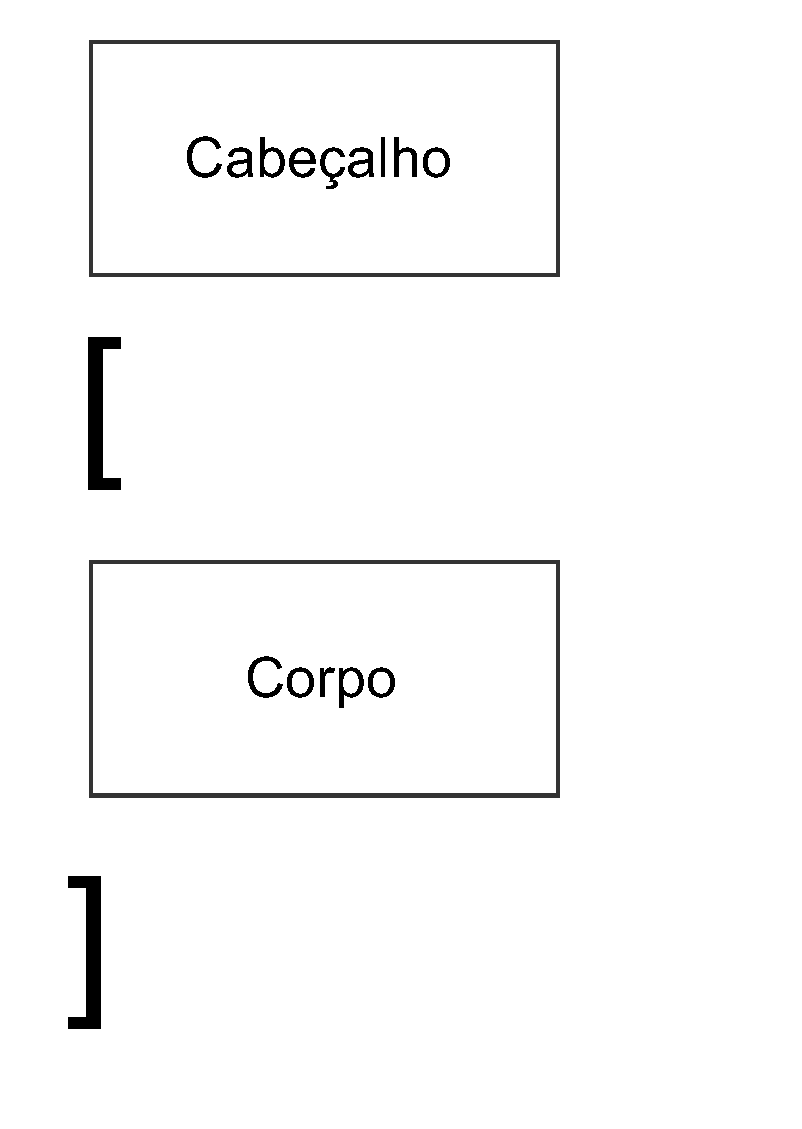
\includegraphics[scale=0.25]{metodologia/figuras/estruturaAgente.pdf}
	\caption{Nó instalado em um veículo.}
	\label{fig:estruturaAgente}
\end{figure}

\subsection{Mecanismo validação e recuperação}

Após um nó receber o último colchete (\emph{]}) ou 500 ms com um agente incompleto o mecanismo de validação e recuperação é ativado. A principal função deste mecanismo é tentar recuperar o agente danificado e se não conseguir descarta-lo. 

A validação verifica se todas as instruções têm cinco caracteres, se a primeira letra é maiúscula e o último caractere é um número, além de verificar as instruções ele válida a estrutura do corpo. Quando alguma instrução não atende uma das três características mencionadas anteriormente ou o corpo não atende o padrão, o mecanismo de recuperação entra em ação. 

Se o erro for no \emph{cabeçalho}, o algoritmo verifica o tamanho da instrução se for maior que cinco ele descartar o agente. Se for menor ele confere a primeira letra se ela atender algumas das instruções suportadas ele recupera colocando a instrução correta. Se não conseguir através do primeiro caractere a próxima tentativa é o último caractere que deve ser um número. Se nenhuma das tentativas forem alcançadas o agente é descartado. A Figura \ref{fig:estruturaInstrucao} demonstra a estrutura da instrução utilizado neste trabalho.

\begin{figure}[htbp]
	\centering
	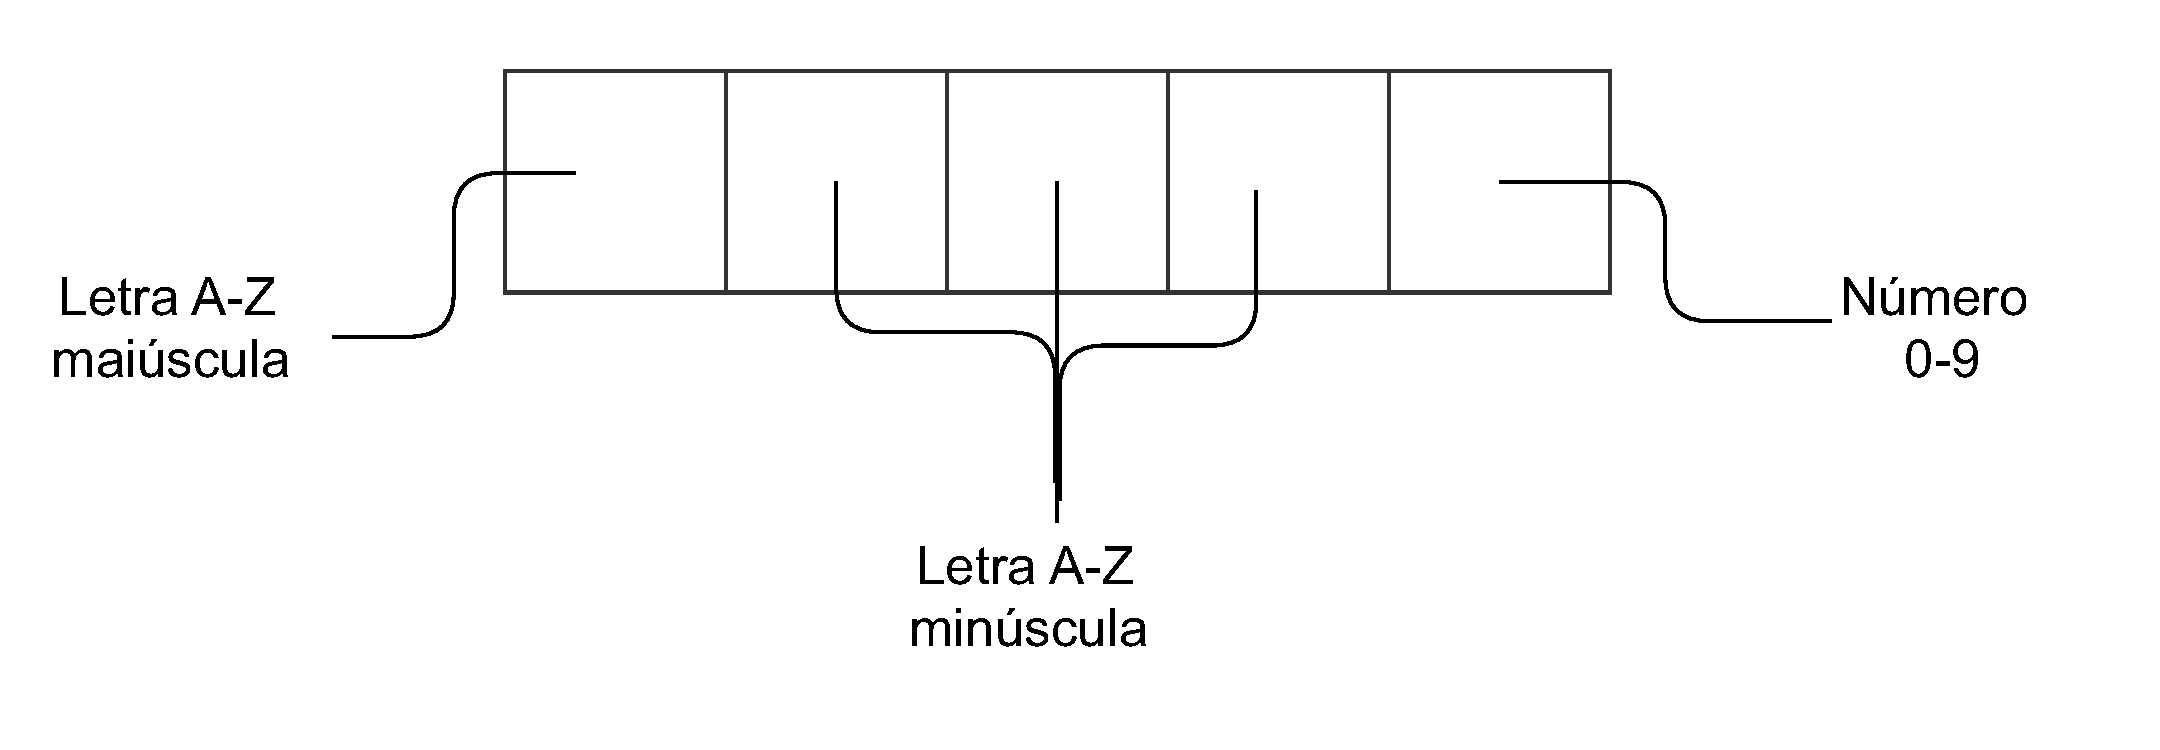
\includegraphics[scale=0.27]{metodologia/figuras/estruturaInstrucao.pdf}
	\caption{Estrutura da Instrução.}
	\label{fig:estruturaInstrucao}
\end{figure}

Para tentar recuperar o corpo, primeiro verifica se existe um caractere de colchete (\emph{[}) iniciando o corpo, se não existir o agente é descartado. Se existir é verificado se o último caractere é um colchete finalizando a estrutura, se não existir o mecanismo coloca o caractere que representa fim. Esse roteiro é reproduzido pelo Algoritmo \ref{lst:mecanismoValidacaoRecuperacao} e a Figura \ref{fig:exemploCodigoAgente} apresenta o agente utilizado neste trabalho.

\begin{algorithm}
	\scriptsize
	\Inicio{
		\Entrada{Agente}
		$instrucoes = agente.pegarInstrucoes()$\;
		$i \gets 0$\;

		\uIf{agente.contem([)}{
			\Repita{$i < instrucoes.quantidade$}{
				$instrucao \gets instrucao[i]$ \;
				\uIf{$instrucao.tamanho < 5$}{
					\uIf{verificar(instrucao.primeiroCaracter)}{
						$instrucao \gets recuperar(instrucao.primeiroCaracter)$\;
					}
					\Else{
						\uIf(verficar(instrucao.ultimoCaracter)){
							$instrucao \gets recuperar(instrucao.ultimoCaracter)$\;
						}
						\Else{
							agente.remover()\;
						}
					}
					
				}
				\Else{
					agente.remover()\;
				}
				i++\;
			}
			\uIf{$agente.ultimoCaracter \neq ]$}{
				$agente.ultimoCaracter \gets ]$
			}
		}
		\Else{
			agente.remover()\;
		}
	}

		
	\caption{Mecanismo validação e recuperação.}
	\label{lst:mecanismoValidacaoRecuperacao}
\end{algorithm}

\begin{figure}[htbp]
	\centering
	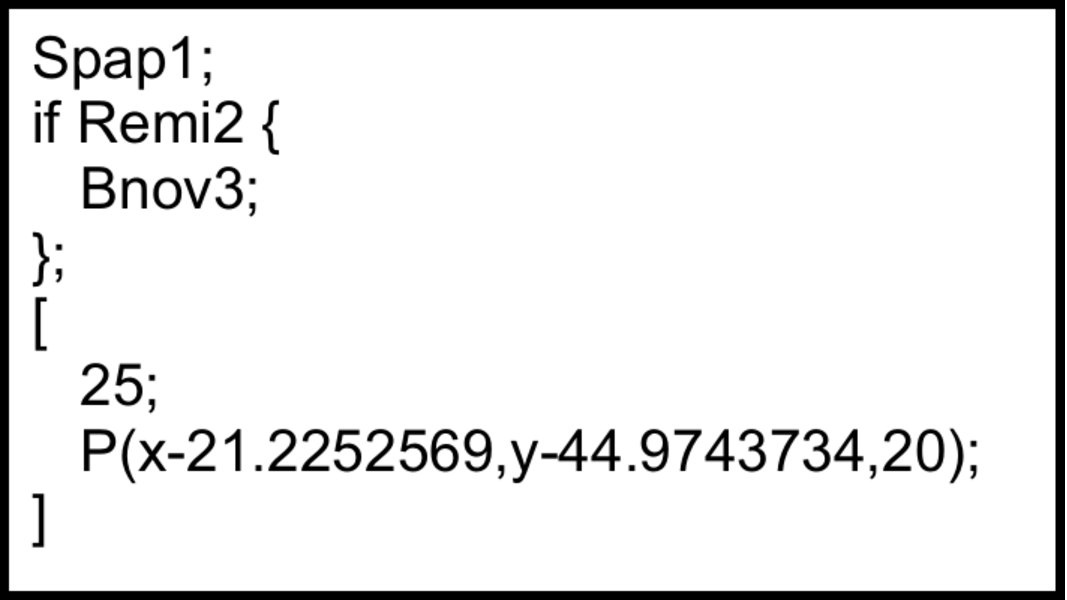
\includegraphics[scale=0.3]{metodologia/figuras/exemploCodigoAgente.pdf}
	\caption{Agente Software.}
	\label{fig:exemploCodigoAgente}
\end{figure}

\subsection{Trajeto e cenário}

Como trajeto é utilizada a avenida norte que está localizada no campus da Universidade Federal de Lavras. O trajeto pode ser visualizado na Figura \ref{fig:trajetoExperimento}. Nesse trajeot o veículo percorre 344,45 metros. 

\begin{figure}[htbp]
	\centering
	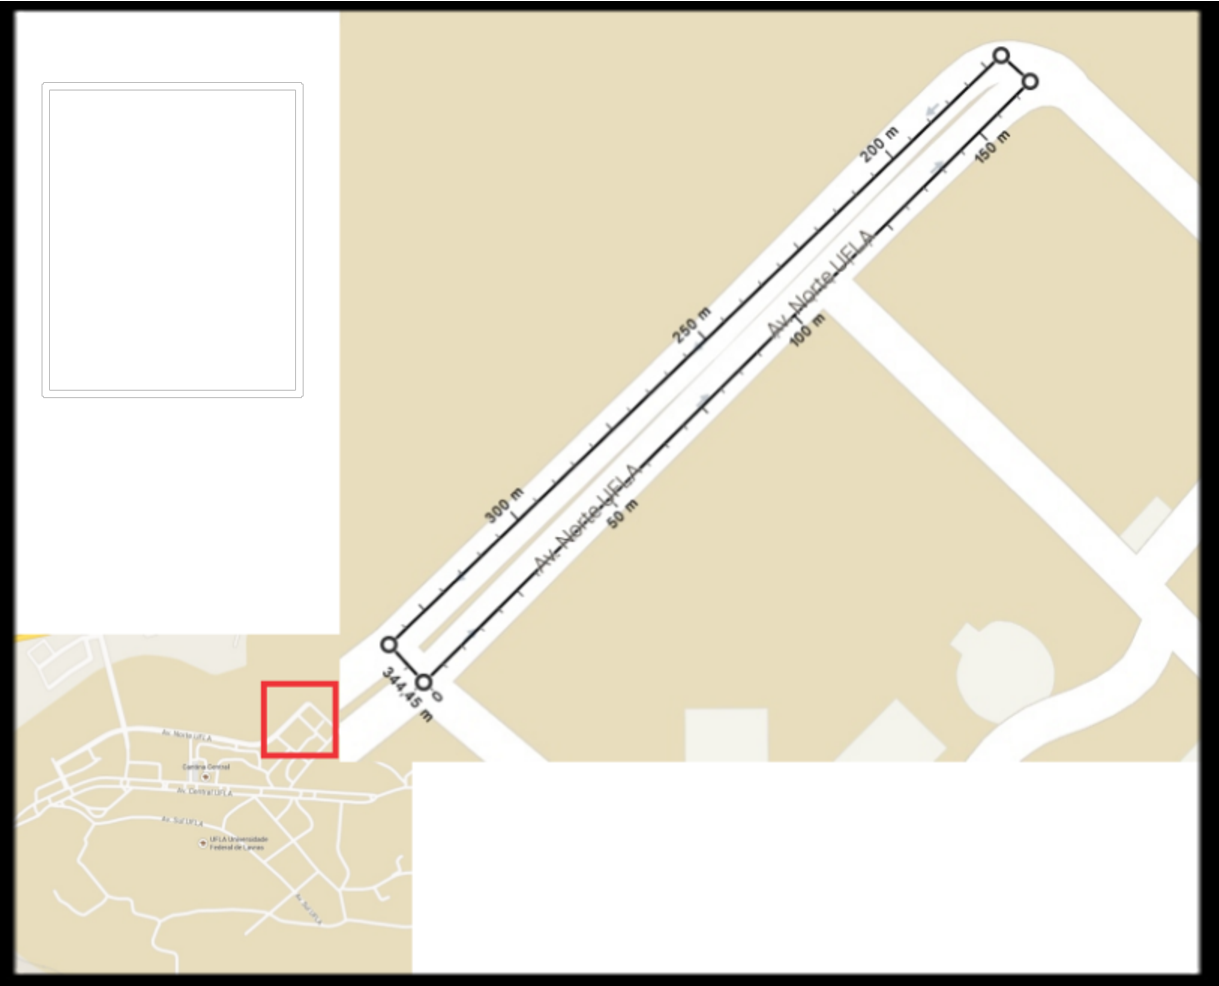
\includegraphics[scale=0.4]{metodologia/figuras/trajetoExperimento.pdf}
	\caption{Modelo de cidade utilizado.}
	\label{fig:trajetoExperimento}
\end{figure}

Os veículos trafegam sobre o roteiro em velocidade média de 20 km/h, a Figura \ref{fig:veiculosUtilizadoExperimento} pode-se visualizar os veículos utilizados no experimento. Existem dois cenários para realizar o experimento, sendo o primeiro caso com infraestrutura e outro somente com veículos. A infraestrutura está localizada ao centro do trajeto como demonstra a Figura \ref{fig:infraestruturaUtilizadoExperimento}.

\begin{figure}[htbp]
	\centering
	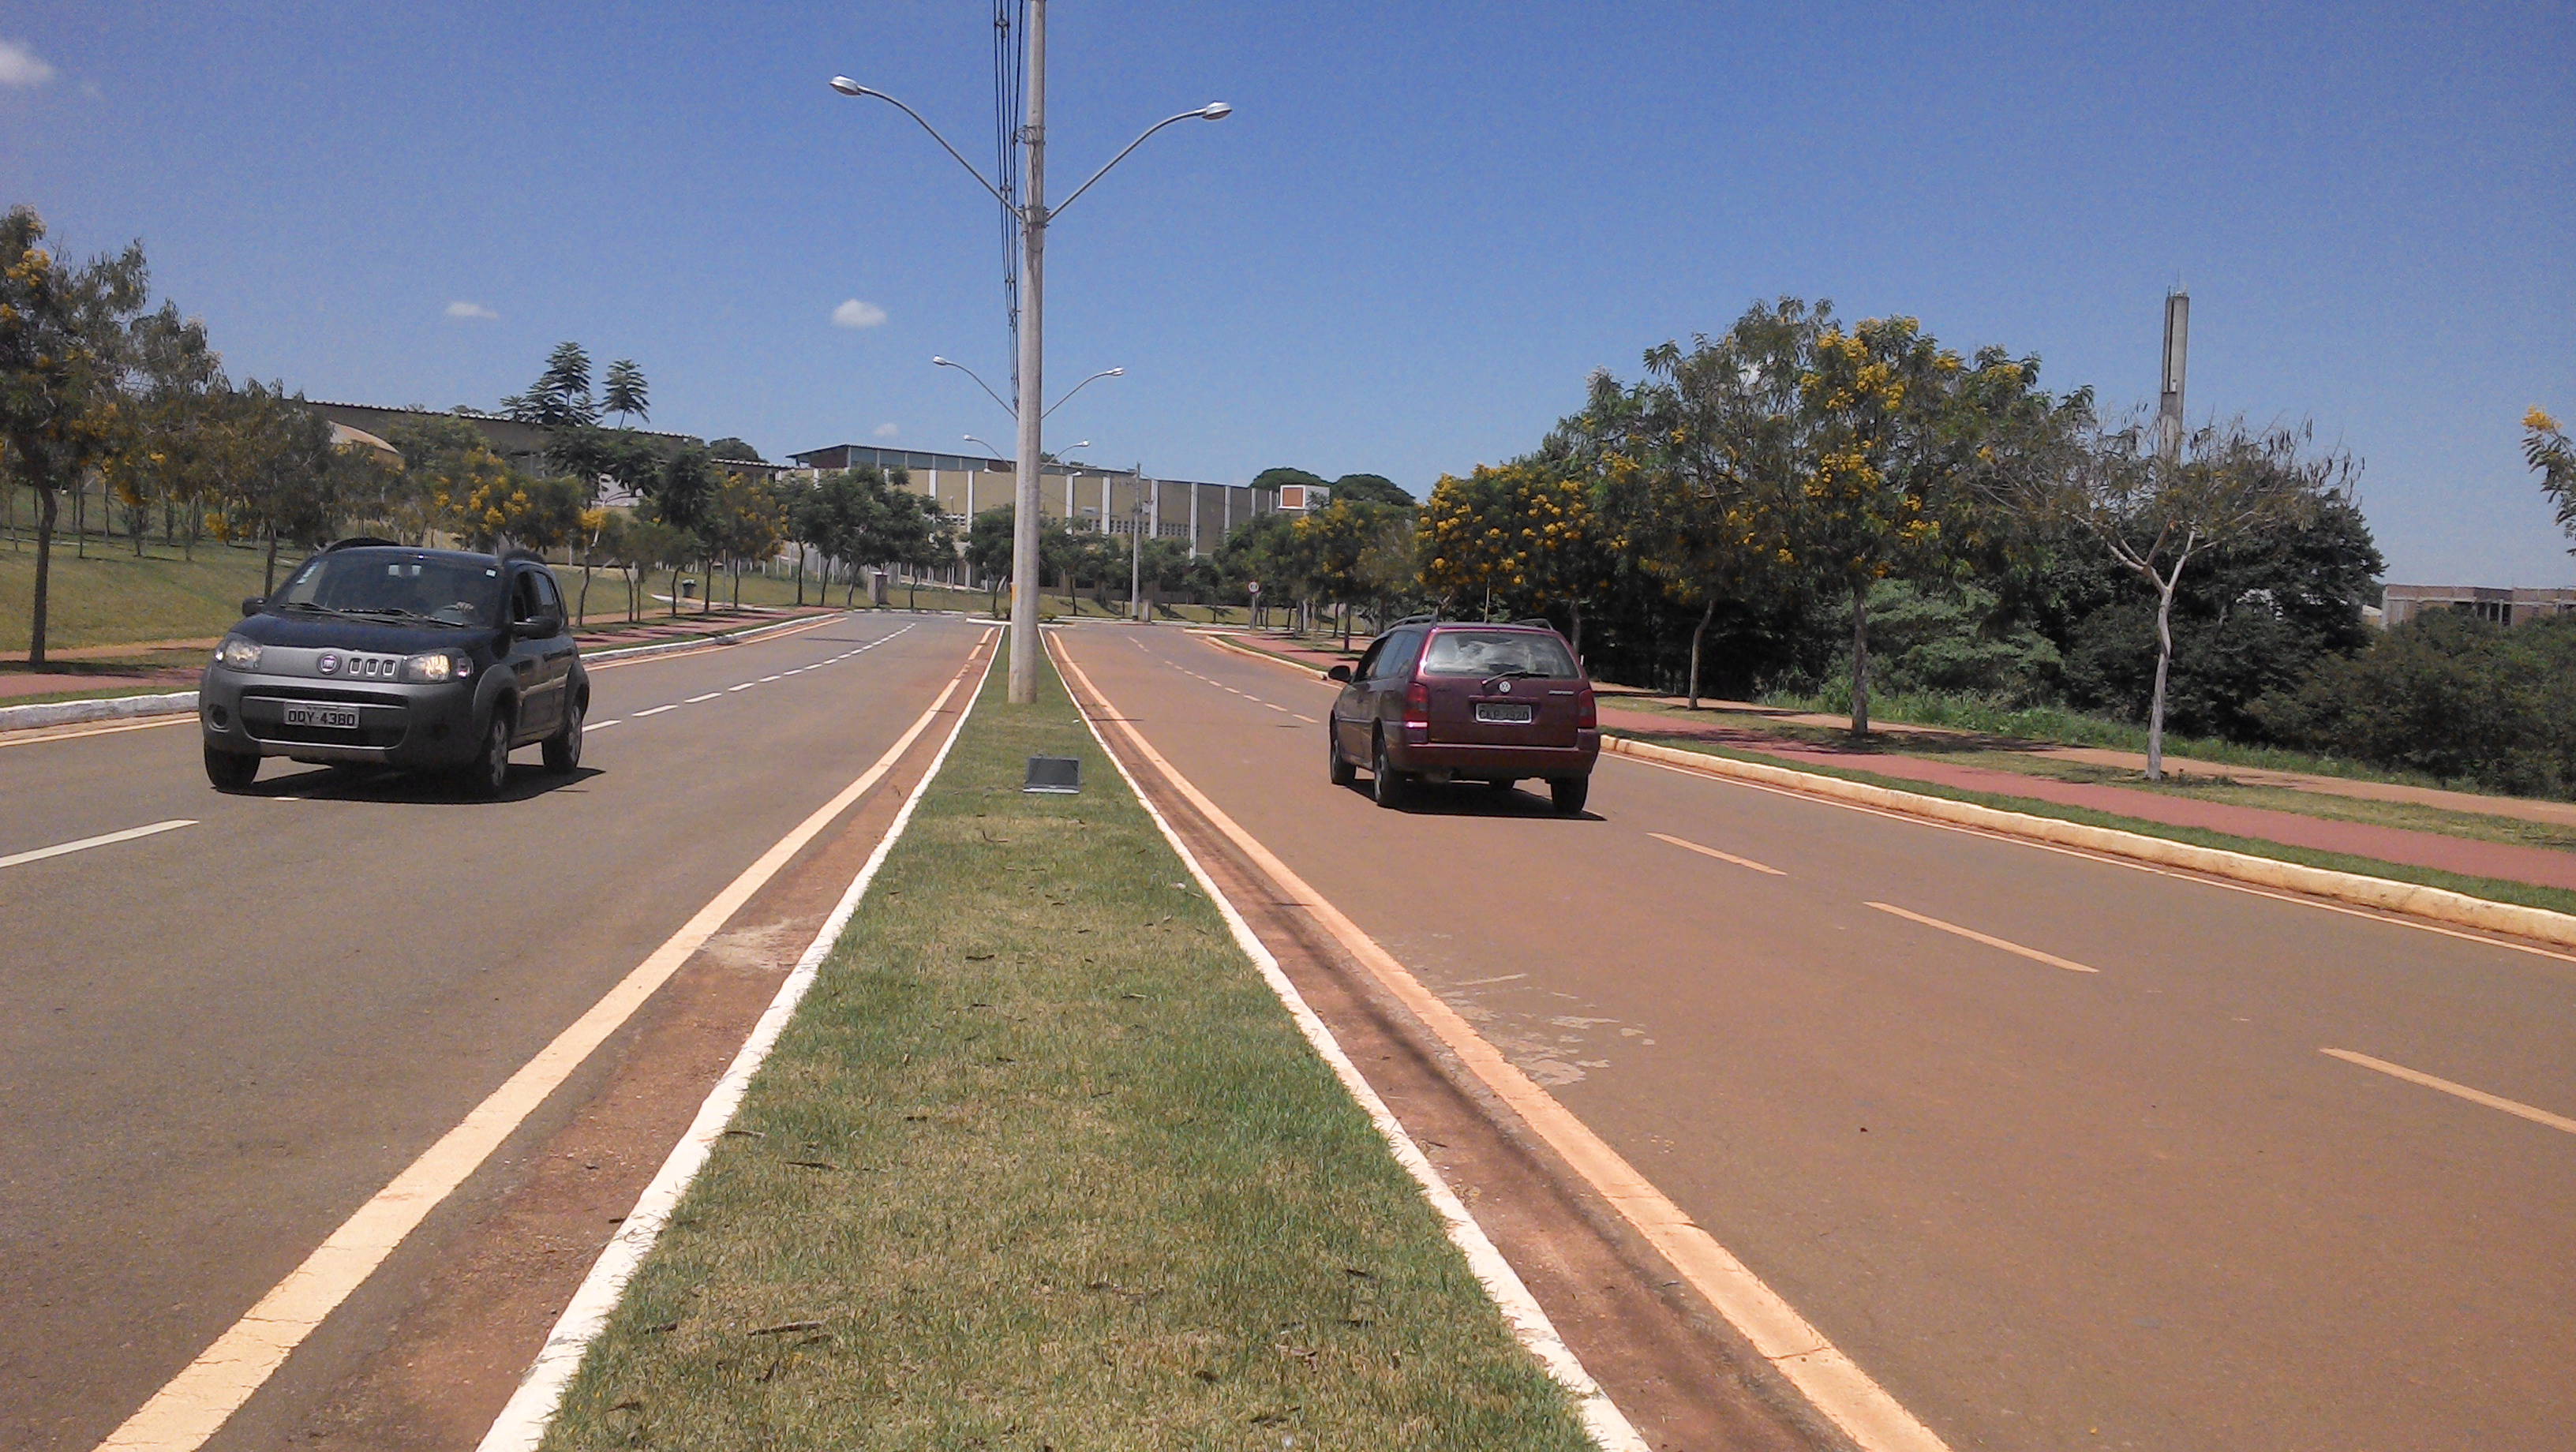
\includegraphics[scale=0.06]{metodologia/figuras/veiculosUtilizadoExperimento.jpg}
	\caption{Veículos utilizados no experimento.}
	\label{fig:veiculosUtilizadoExperimento}
\end{figure}

A infraestrutura é colocada aproximadamente ao centro do cenário. Quando a infraestrutura não é utilizada ela é desligada. A infraestrutura tem a função de receber e armazenar o agente até um novo nó se aproximar. Para saber que o agente passou pela infraestrutura é adicionado um caractere \emph{I} ao corpo do agente. Esse caractere vai auxiliar no cálculo da quantidade de vezes que o agente passou pela infraestrutura.

\begin{figure}[htbp]
	\centering
	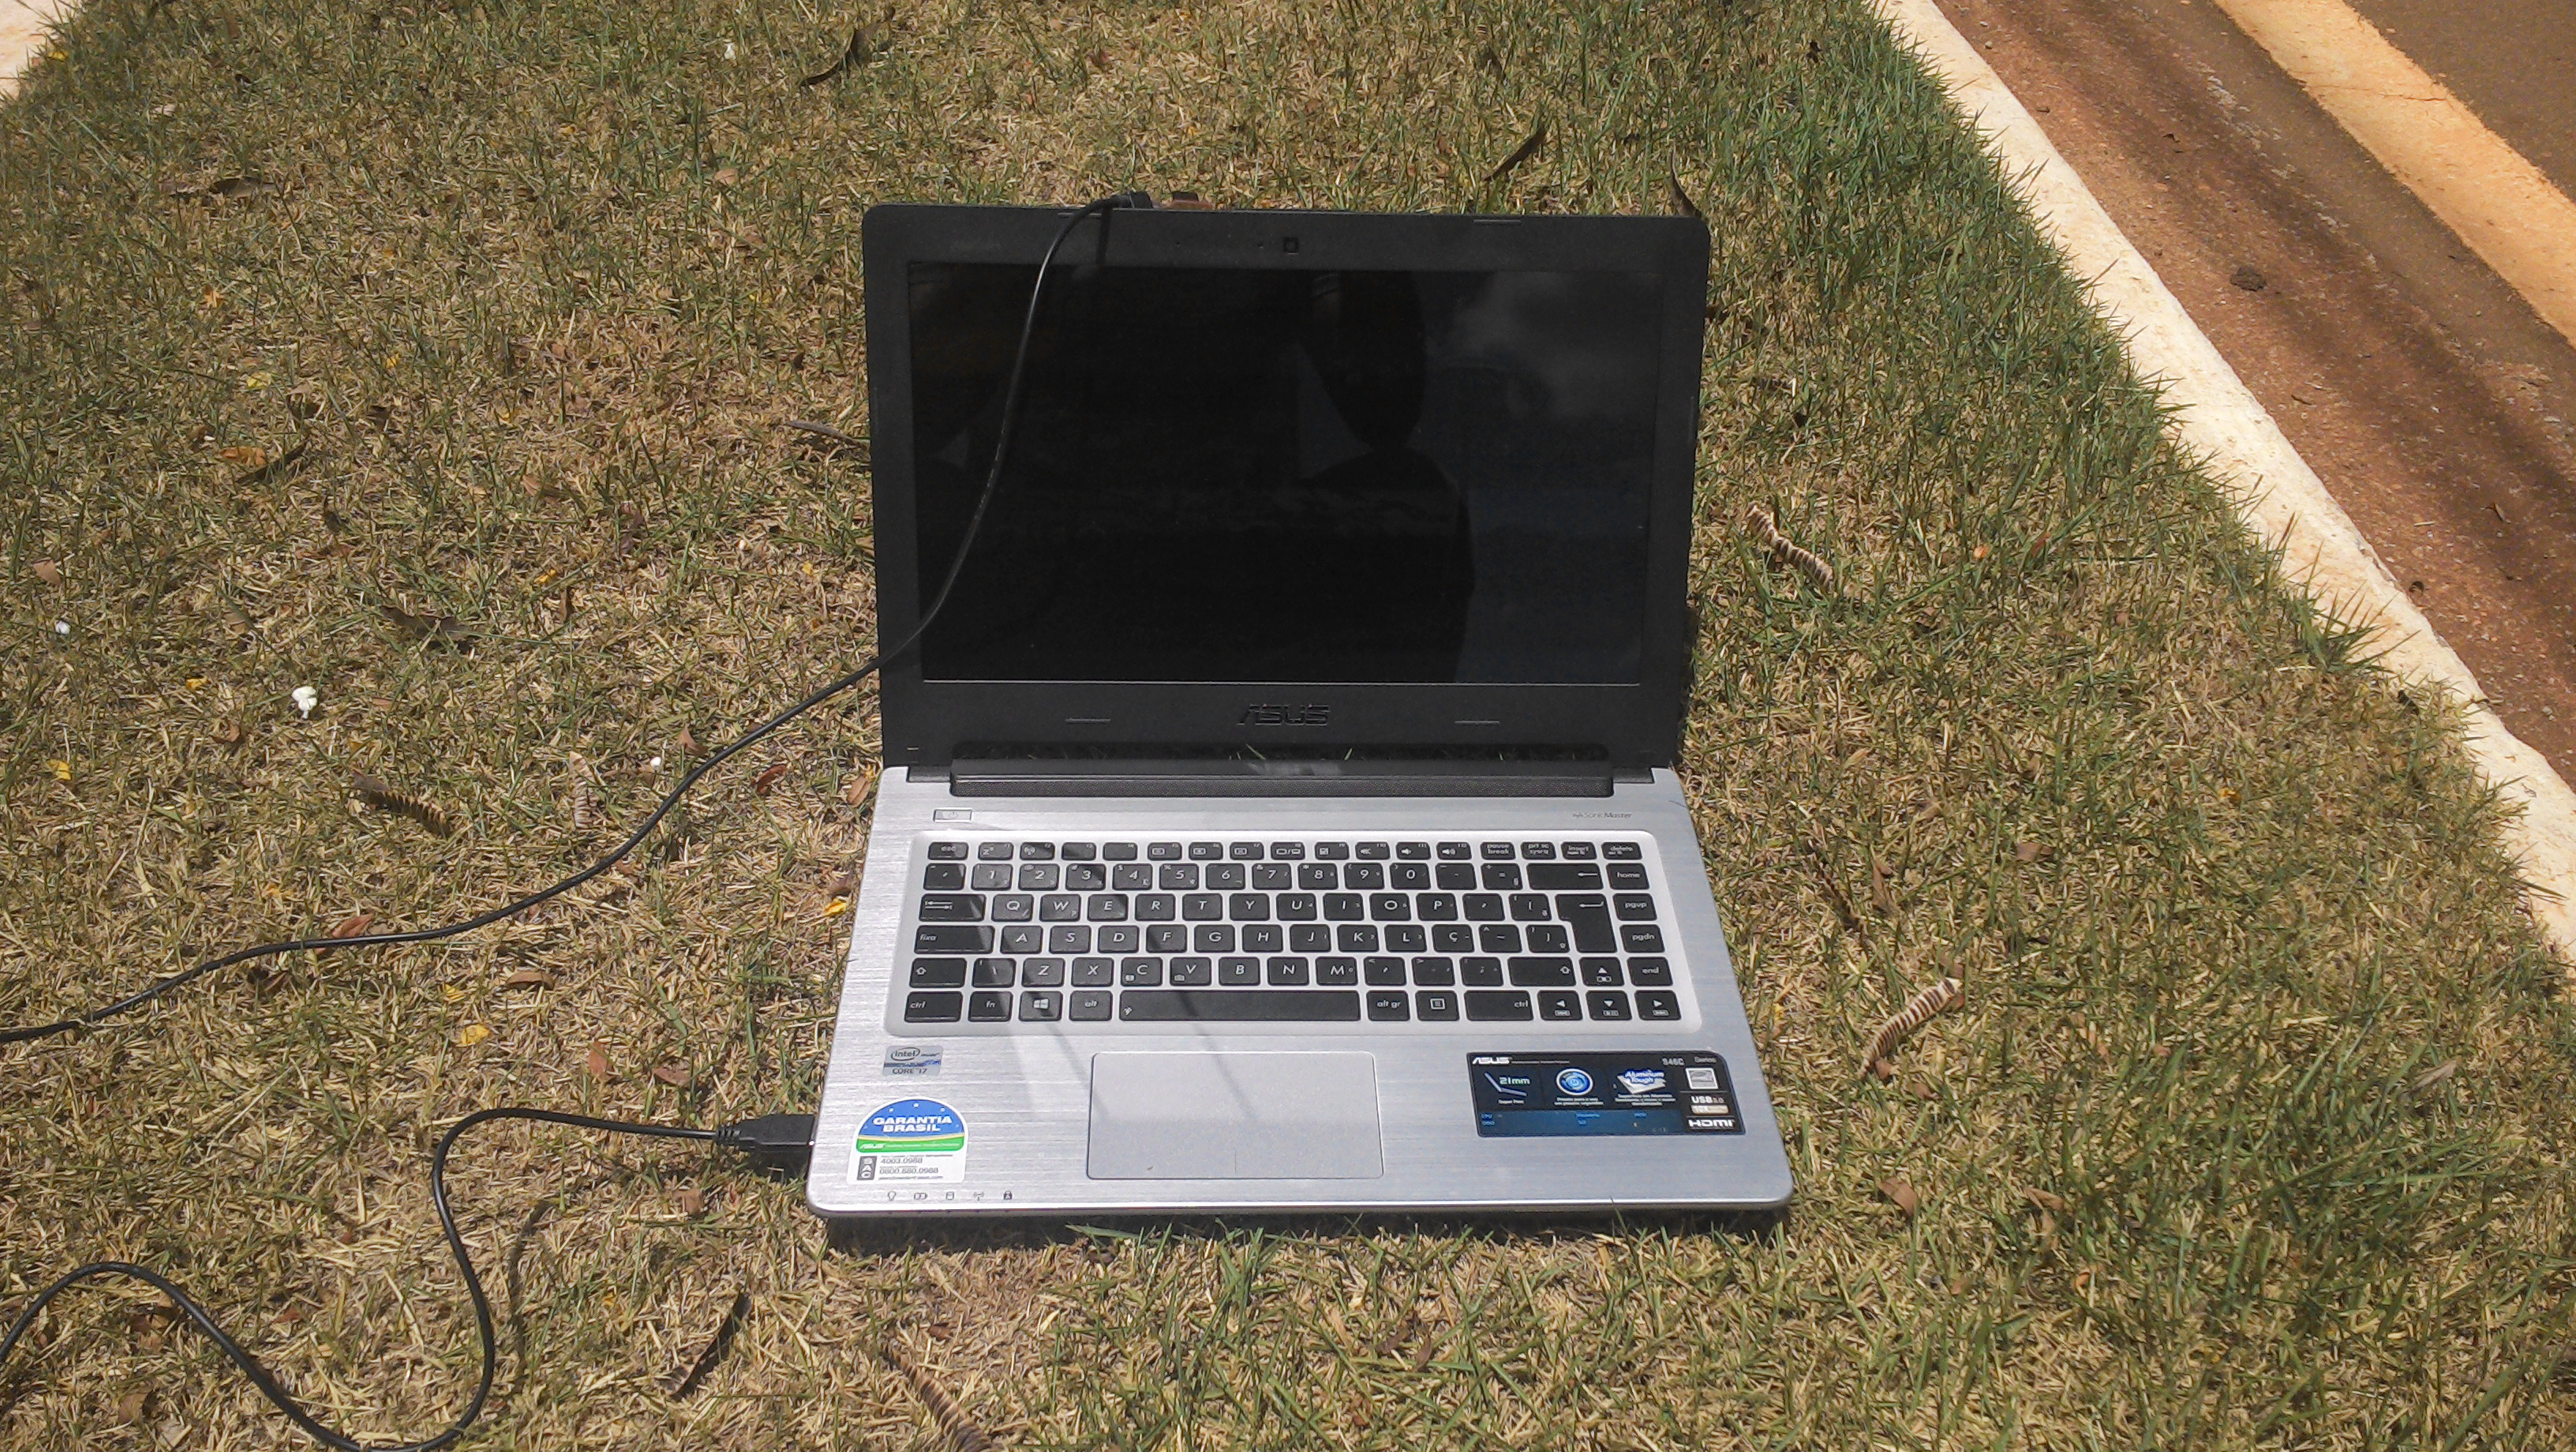
\includegraphics[scale=0.06]{metodologia/figuras/infraestruturaUtilizadoExperimento.jpg}
	\caption{Infraestrutura utilizada no experimento.}
	\label{fig:infraestruturaUtilizadoExperimento}
\end{figure}

No experimento realizado, cada veículo percorreu cinquenta vezes o trajeto, vinte e cinco com a infraestrutura ativada e vinte e cinco com a infraestrutura desativada. Foram recolhidas informações sobre a latência e taxa de perda do agente. Ao fim dessa fase foram calculados o desvio padrão, variância e os resultados foram analisados.


